\documentclass[11pt,a4paper,openright,twoside]{report}
\usepackage[utf8]{inputenc}
\usepackage{amsmath}
\usepackage{amsfonts}
\usepackage{amssymb}
\usepackage{graphicx}
\usepackage{geometry}
\usepackage{caption}
\usepackage{float}
\usepackage{subcaption}
\usepackage{hyperref}
\usepackage{afterpage}

\setlength{\parindent}{0em}
\setlength{\parskip}{0.5em}

\geometry{
 a4paper,
 total={170mm,257mm},
 left=20mm,
 top=12mm,
}

\newcommand{\ZZ}{$ZZ\to ll\nu\nu$ }
\newcommand{\Zg}{$Z\gamma\to ll\gamma$ }
\newcommand{\llM}{$ll+E_T^{miss}$ }
\newcommand{\met}{$E_T^{miss}$ }
\newcommand\blankpage{%
    \null
    \thispagestyle{empty}%
    \addtocounter{page}{-1}%
    \newpage}    

\begin{document}
\begin{titlepage}
\centering

\includegraphics[width=0.9\linewidth]{Title_Head.png}
\vfill
{\Huge Estimating \ZZ background in the \llM final state using \Zg data\\\vspace{1cm}\Large A Thesis \\}
\vspace{1cm}
{\Large submitted to\\Indian Institue of Science Education and Research, Pune\\ in partial fulfillment of the requirements for the \\BS-MS Dual Degree Programme\vspace{1cm}\\by\vspace{1cm}\\Mangesh Sonawane\vspace{0.2cm}\\Registration Number: 20121083\\}
\vspace{1cm}

\includegraphics[scale=0.8]{iiser_logo.png}
\vfill
{\Large Indian Institute of Science Education and Research, Pune\vspace{0.1cm}\\Dr. Homi Bhabha Road,\vspace{0.3cm}\\ Pashan, Pune 411008, INDIA}
\vfill
\vfill
\end{titlepage}
\pagestyle{empty}
\begin{center}
{\large June 2017 - April 2018\\}
\vspace{10cm}
\large 
Conducted at : DESY\\
Notkestra\ss e 85,\\
22607, Hamburg\\
Germany\\
\vspace{10cm}
Supervisor: Dr. Beate Heinemann\\
\copyright Mangesh Sonawane 2018\\
All rights reserved
\vfill
\newpage
\Huge \textbf{Certificate\\}
\end{center}
\vspace{1cm}
\normalsize This is to certify that this dissertation, entitled "Estimating \ZZ background in the \llM final status using \Zg data", submitted towards the partial fulfilment of the BS-MS dual degree programme at the Indian Institute of Science Education and Research (IISER), Pune, represents the work carried out by Mangesh Sonawane at the Deutsches Elektronen-Synchrotron (DESY), Hamburg, under the supervision of Dr. Beate Heinemann, Professor of Experimental Particle Physics at the Institute of Physics, University of Freiburg, during the academic year 2017-2018.
\vfill
\begin{center}
Mangesh Sonawane\hspace{8cm}
Dr. Beate Heinemann
\end{center}
\vfill
Committee:\\
Dr. Beate Heinemann\\
Dr. Seema Sharma
\vfill
\vfill
\newpage
\blankpage
\newpage
\topskip0pt
\vspace*{\fill}
\noindent I dedicate this thesis to my parents, Avinash and Ranjana Sonawane, my mentors, Dr. Sourabh Dube and Dr. Seema Sharma, and to my friends and colleagues and IISER, without whose timely advice and support this thesis would not have been made possible.
\vspace*{\fill}
\newpage
\blankpage
\newpage
\begin{center}
\Huge \textbf{Declaration\\}
\end{center}
\vspace{1cm}
\normalsize I hereby declare that the matter containined within the thesis entitled "Estimating \ZZ background in the \llM final status using \Zg data", contains the results of the work carried out by me at the Deutsches Elektronen-Synchrotron (DESY) Hamburg, under the supervision of Dr. Beate Heinemann, and the same has not been submitted elsewhere for any other degree.
\vfill
\begin{center}
Mangesh Sonawane\hspace{8cm}
Dr. Beate Heinemann
\end{center}
\vfill
Committee:\\
Dr. Beate Heinemann\\
Dr. Seema Sharma
\vfill
\vfill
\newpage
\blankpage
\newpage
{\Huge \textbf{Acknowledgements\vspace{2cm}\\}}
I would like to express my deepest gratitude for Dr. Beate Heinemann for her guidance and patient mentoring. It's not just technical skills that I have acquired under her supervision, but also an understanding of how a physicist approaches the subject and tackles the inevitable problems that surface.\vspace{1cm}

$\langle$ placeholder $\rangle$

\newpage
\blankpage
\newpage

\chapter*{Abstract}
\addcontentsline{toc}{chapter}{Abstract}
\pagenumbering{roman}
\setcounter{page}{1}
In the search for Dark Matter (DM) at the LHC, SM particles are produced in association with DM particles, which are invisible as they don't interact with the detector. Thus events with large imbalance in transverse momentum are of interest. One such signature is $ll + E_T^{miss}$. The dominant background contributing to the search for DM in the $ll + E_T^{miss}$ is $ZZ \rightarrow ll\nu\nu$.  Currently, this background is determined using Monte Carlo simulation, with an uncertainty of $\approx 10\%$ \cite{ZH_ATLAS}. The goal of this study is to establish a data driven method to estimate this background, and reduce the uncertainty. Using \Zg, which is a process with low backgrounds and has a high $BR*\sigma$, it is possible to estimate the \ZZ contribution. In regions where $p_{T}(\gamma) \gg M_{Z}$, the two processes are kinematically similar. They have the same production mechanisms, but differ due to the photon and Z boson couplings to the quarks being different, as well as the difference in mass (photons are massless, while Z bosons are massive). Introducing a transfer factor $R$ as the ratio $\sigma(ZZ)/\sigma(Z\gamma)$ which is determined from simulation, the contribution of \ZZ to the background can be estimated from \Zg data. The uncertainty on the prediction of $R$ due to theoretical aspects is estimated in this work.
\thispagestyle{plain}
\tableofcontents
\thispagestyle{empty}
\cleardoublepage
\pagenumbering{arabic}
\chapter{Introduction}
\setcounter{page}{1}

The Standard Model of physics is one of the most successful theories developed, describing the fundamental particles and their interactions. It is theoretically self-consistent, and has enjoyed tremendous success in providing stunningly accurate experimental predictions. However, the Standard Model is not complete theory of fundamental interactions. It does not provide an explanation for several observed phenomena, such as gravity, or the accelerating expansion of the universe, among others.

One such question that triggers burning curiosity is the apparent incongruity of galaxy rotation curves with the theory of Newtonian mechanics: stars in the arms of spiral galaxies appear to move much faster than Newtonian physics would predict. Either the current understanding of mechanics is incomplete, or there is more mass present somewhere in the galaxy that is not visible by any method that is currently employed. This invisible hunk of matter is what is termed as Dark Matter (DM).

Detailed observations of these rotation curves, along with measurements of other phenomena such as gravitational lensing by distant galaxies, galaxy clusters, and Cosmic Microwave Background (CMB) lead to the conclusion that, if the Dark Matter hypothesis is true, the amount of visible Baryonic matter in the universe is a mere 4\%. The remaining 96\% of the universe is composed of Dark Matter and Dark Energy.

Now it becomes important to address the question: what exactly is Dark Matter? 

Several extensions to the Standard Model, called Beyond Standard Model (BSM) theories, attempt to provide an explanation of these observed phenomena. Dark Matter hasn't been observed to interact directly through the electromagnetic force, and are thus invisible to current detectors. Consequently candidates for Dark Matter are called Weakly Interacting Massive Particles (WIMPs). In LHC experiments, events with WIMPs in the final state show up as an imbalance in the momentum in the plane transverse to the beam (referred to as \met throughout this thesis).

One such BSM theory postulates that these Dark Matter candidate particles may couple to Standard Model particles in interactions mediated by the Higgs boson. Fig \ref{fig:higgs} illustrates some of the possible processes for the production of the Higgs boson. The Higgs boson can then decay into invisible particles.

\begin{figure}[H]
\centering
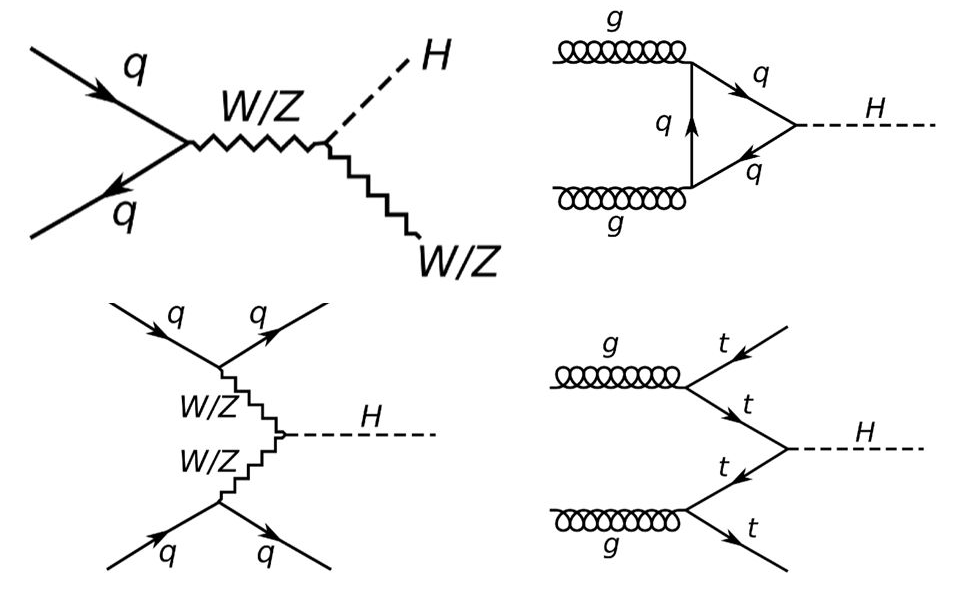
\includegraphics[width=0.5\linewidth]{higgs_production.png}
\caption{Feynman diagrams for the Standard Model production of the Higgs boson; VH: Higgs produced in association with a $W/Z$ boson (top left), ggF: gluon-gluon fusion (top right), VBF: vector boson fusion (bottom left), ttH: (bottom right). The Higgs boson then further decays into invisible DM particles.}
\label{fig:higgs}
\end{figure}

In this thesis, a closer look is taken at the VH channel, in particular ZH, where the Higgs boson decays invisibly into DM particles, and the $Z$ boson decays into a dilepton pair. The signature of such a process is \llM. A possible search in this channel would constitute stacking all known Standard Model processes that contribute to the \llM signal (making up the background) and look for excesses in data which will indicate the presence of non-Standard-Model processes. In this thesis, a closer look is taken at the \ZZ process, which constitutes the dominant SM background in the \llM final state. However, it is difficult to discriminate between the Standard Model \ZZ and $ZH\to l^+l^-+E_T^{miss}$, the process under consideration, because of the identical final state. Thus, an attempt is made to estimate it using alternate processes with clean signals.

\section{The Standard Model}
The Standard Model is the name given to the theory of particles, fundamental forces, and interactions that govern the Universe. It describes three of the four forces: the electromagnetic, strong and weak forces. Figure \ref{fig:SM} shows a schematic representation of the elementary particles in the Standard Model.

The Standard Model classifies fundamental particles as either Fermions or Bosons:
\begin{itemize}
\item \textbf{Fermions:} make up the matter in the universe. Fermions are spin 1/2 particles, and are categorized into quarks and leptons. Quarks exist in 6 flavors, up, down, charmed, strange, top (or truth) and bottom (or beauty). Leptons too exist in 6 flavors: electrons, muons, and taus, and their respective neutrinos. The up, charmed and top quarks carry an electric charge of +2/3e. The down, strange and bottom quarks carry an electric charge of -1/3e. The electron, muon and tau carry an electric charge of -1e, and the neutrinos carry no electromagnetic charge. Here, e is the unit of electromagnetic charge, and is equal to $1.602\times 10^{-19}$ Coulombs. Quarks and leptons are divided into three generations, with each generation having more mass than the last. Each fermion has a parity inverted counterpart, called an anti-particle, having the same mass, but an opposite charge. For example, an anti-electron (or a positron) has a charge of +1e and a down anti-quark will have charge of +1/3e.
\item \textbf{Bosons:} are particles with integral spin that mediate the interactions between particles in the universe. There are four gauge bosons: the photon, which mediates electromagnetic interactions, the $W$ and $Z$ bosons that mediate weak interactions, and the gluons, which mediate strong interactions. These are vector bosons, having spin +1. In addition, there is a scalar boson (spin 0), the Higgs boson, which gives particles their mass.
\end{itemize}
\begin{figure}[h]
\centering
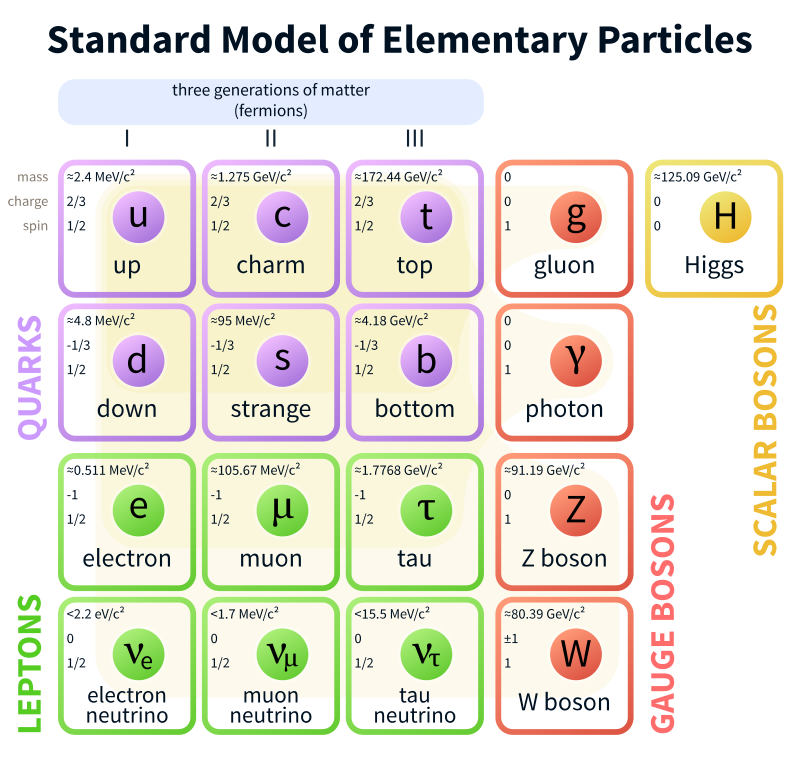
\includegraphics[width=0.7\linewidth]{standard_model.png}
\caption{A schematic representation of the Standard Model\cite{SM} of particles. The table shows the three generations of fermions (classified as quarks and leptons) that are the building blocks of all known matter in the Universe, and bosons that mediate interactions, and are thus responsible for 'forces'}
\label{fig:SM}
\end{figure}
The Standard Model addresses three of the four fundamental forces; it does not address the Gravitational force. The strong, weak and electromagnetic forces can be described by the SU(3)$\times$SU(2)$\times$U(1) local gauge symmetry group, where the SU(3) symmetry group describes the strong interaction, and the electroweak interactions are based on the SU(2)$\times$U(1) symmetry group. There are 8+3+1 generators associated with this model, each generator corresponding to a vector boson. 

Thus, there are 8 gluons, which are massless spin 1 particles with an intrinsic property called color charge, that mediate strong interactions (described by Quantum Chromodynamics). They are responsible for interactions between quarks (leptons do not interact via the strong force) as quarks have a non vanishing color charge. At low energies, quarks cannot be found in isolation, instead occurring in triplets called $Baryons$, such as protons, or a bound quark-antiquark pair, called $Mesons$. This is because of color confinement\cite{confinement}.

The interaction of the scalar Higgs field with the vector fields $W^+$, $W^-$, $W^0$ and $B$ causes the spontaneous breaking of the SU(2)$\times$U(1) symmetry, resulting in 3 massive and one massless gauge boson. It also implies the existence of a neutral scalar boson, known as the Higgs boson, which was discovered in July 2012\cite{Higgs}. The generators of SU(2)$\times$U(1) correspond to the $W^+$,$W^-$ and $Z$ bosons, massive vector bosons(spin 1) that mediate weak interactions, and the massless vector boson $\gamma$ (photon), which mediates electromagnetic interactions. The $W$ bosons are charged, whereas the $Z$ boson and $\gamma$ are neutral.

\section{Inadequacies of the Standard Model}
Despite its immense success, the Standard Model does not paint a complete picture of everything that we observe. It does not account for several phenomena that are experimentally observed, such as:
\begin{itemize}
\item Gravity: The Standard Model does not include gravity. If, analogous to the other forces, a 'graviton' is introduced into the Standard Model as an extension, it does not describe what is observed experimentally. In fact, the Standard Model is incompatible with general relativity.
\item Dark Matter and Dark Energy: There are cosmological observations which do not match predictions based on the visible amount of mass in the universe. A fit with the observations predicts additional invisible matter, called Dark Matter. Similarly, the universe is expanding at an accelerating rate, which hints at the existence of Dark Energy. The Standard Model does not account for exotic matter such as these. In fact, the Standard Model only accounts for about 4\% of the content of the universe.
\item Neutrino masses: Neutrinos are taken to be massless in the Standard Model. However, neutrino observations have been observed, which is only possible if neutrinos have mass.
\item Matter-antimatter asymmetry: According to the Standard Model, matter and antimatter should be created in equal quantities. However, the universe appears to have a preference for matter, indicating that in its initial state of the universe, this symmetry was broken.
\item Hierarchy problem: Quantum corrections to the Higgs mass are divergent, and force it to be very large. However, experiments show a surprisingly small number for the Higgs mass, at 125 GeV. There appear to be some extraordinary fine tuned cancellations that make this mass so small.
\end{itemize}

The Standard Model is incomplete, and thus requires modifications or additions to it, which are collectively called Beyond Standard Model (BSM) theories.

\subsection{Beyond the Standard Model}
Several extensions to the Standard Model have been proposed that attempt to address some of its inadequacies. 

Supersymmetry (SUSY) attempts to reconcile gravity with the SM, and adds another symmetry to the Standard Model, predicting the existence of $supersymmetric$ partners, called sparticles, to Standard Model particles. For example, sleptons are supersymmetric partners to the corresponding leptons, and differ by spin 1/2. SUSY would also resolve the hierarchy problem by ensuring that the divergences would cancel out at all orders in the perturbation expansions, if the superpartners have mass near the electroweak scale (broadly, between 100 and 1000 GeV).

The observation of neutrino oscillations imply that neutrinos have mass, however, these observations can only reveal the mass difference between the different neutrino flavors. The absolute mass of the neutrinos has been constrained to have an upper limit of 2 eV, much smaller than the lightest SM particles, by precision measurements of tritium decays. To incorporate neutrino masses, an extension to the Standard Model, the see-saw mechanism, introduces right handed neutrinos and couples them to left-handed neutrinos with a Dirac mass term.

Both SUSY and the addition of a sterile right-handed neutrino to the SM are extensions that provide candidates for Dark Matter. These candidates are known as Weakly Interacting Massive Particles (WIMPs). They do not interact electromagnetically, and are thus invisible to most detectors.

\subsection{Dark Matter}
Cosmological observations of galaxies made over the decades, such as the velocity curves of galaxies (called galaxy rotation curves) indicate an anomaly; the stars in the arms of spiral galaxies appear to move faster than what would be expected from Keplerian relations, using the visible mass from the galaxies. Figure \ref{fig:grc} shows the two rotation curves, expected and observed, of NGC 6503, a field\footnote{Field galaxies do not belong to a large cluster, and are thus gravitationally isolated}  spiral galaxy.\cite{galaxy}
\begin{figure}[H]
\centering
	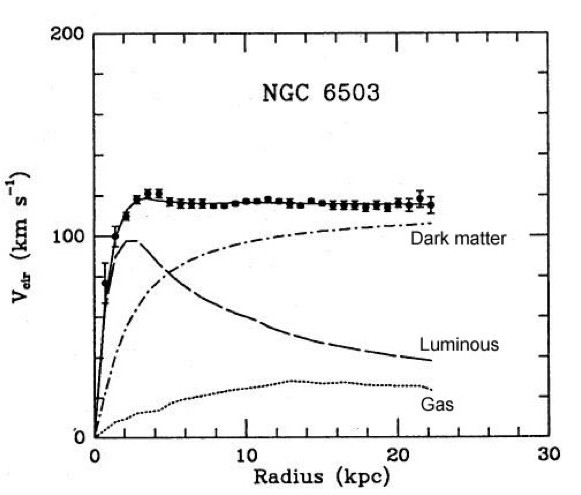
\includegraphics[width=0.7\textwidth]{GRC.jpeg}
	\caption{Velocity of stars in NGC 6503, a field spiral galaxy, as a function of radial distance from the center of the galaxy\cite{galaxy}. The 'Luminous' curve is what would be expected from the visible mass, but what is observed is much higher, indicating excess invisible matter.}
	\label{fig:grc}
\end{figure}
Either the current understanding of Newtonian Mechanics is incomplete, or there is additional mass that is not visible which is contributing to the mass term in Newton's equation. This invisible mass is what is termed as Dark Matter. Ergo, Dark Matter appears to interact gravitationally, but not electromagnetically, with visible (Standard Model) matter. It is possible that Dark Matter is made up of and exotic and hitherto undiscovered kind of matter, and searches are underway at the LHC to look for Dark Matter via its interactions with the Standard Model.

There is additional cosmological evidence supporting Dark Matter, such as gravitational lensing of distant galaxies, structure formation in the early universe, anisotropy in the cosmic microwave background, etc.

\subsubsection{Dark Matter searches at the \hyperref[ch:LHC]{Large Hadron Collider}}
As Dark Matter does not interact electromagnetically, any Dark Matter particles produced in collider experiments will be invisible to detectors at the LHC. Thus, in event reconstruction, such events are expected to be marked by a significant imbalance in transverse momentum (\met). Currently, Dark Matter searches are conducted at the LHC\cite{DM_searches}. Dark Matter particles are denoted by $\chi$.
\begin{itemize}
\item Mono $\chi$ searches : These searches look for the production of a Standard Model particle in association with \met. Figure \ref{fig:Mono_X} shows the Feynman diagrams for the Mono-X processes.
	\begin{itemize}
	\item Mono-jet : In theory, it is possible to produce Dark Matter particles in association with one or more QCD jets from initial state radiation. Thus mono-jet searches look for one or more jets in events with large \met.
	\item Mono-V : In a similar manner to mono-jet searches, a mono-V search looks for a single vector ($\gamma,W$ or $Z$) boson. If DM particles couple directly to a pair of gauge bosons, this may be the dominant mode of DM production.
	\item Mono-Higgs : It may also be that a single Higgs boson is produced in association with \met. Such events would be characterised by a $H\to\gamma\gamma$ or $H\to bb$ final state.
	\end{itemize}
	
\begin{figure}[H]
\centering
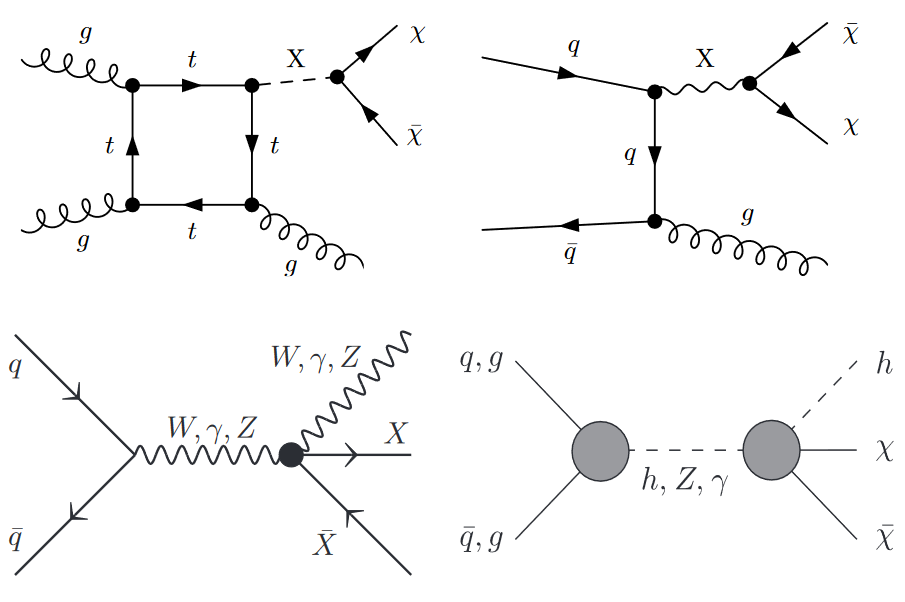
\includegraphics[width=0.65\textwidth]{Mono_X.png}
\caption{Feynman diagrams for mono X processes, showing mono-jet production (top) induced by gluons (top left) and quarks (top right) \cite{mono_j} where the mediator X can be a scalar, pseudo-scalar, vector or axial-vector particle; mono-V (bottom left) \cite{mono_V}; and mono-higgs (bottom right) \cite{mono_h}, where h is the Standard Model Higgs boson with mass 125 GeV.}
\label{fig:Mono_X}
\end{figure}

\item DM+top : If DM particles couple predominantly to heavy quark flavors, a search for a top quark pair is a promising direction to head in.
\item Invisible Higgs :  If the mass of the DM particles is less than half the mass of the Higgs boson, it may be possible that the DM particles couple to the Standard Model via the Higgs boson, i.e $H\to\chi\chi$ processes. The main methods of Standard Model Higgs production are shown in Figure \ref{fig:higgs}.
	\begin{itemize}
	\item Vector boson fusion (VBF): In VBF processes, the Higgs is produced from the interaction of two vector bosons.
	\item Production of Higgs in association with a massive vector boson (VH) : This mechanism, together with VBF are the most important methods of Higgs production in invisible Higgs searches. Such events can be recognised with a large imbalance in transverse momentum, as well as the decay products of the vector boson.
	\item Gluon gluon fusion (ggF) : It is also possible for the Higgs to be produced from the interaction of gluons.
	\end{itemize}
\end{itemize}

This thesis investigates the Standard Model background to the $ll+$\met signal with respect to the production of an invisible Higgs in association with a leptonically decaying gauge boson. Chapter \ref{ch:LHC} gives an overview of the Large Hadron Collider, the ATLAS detector, and details the event topology. Chapter \ref{ch:theory} address the theoretical framework of this thesis.

\chapter{The Large Hadron Collider}\label{ch:LHC}

\pagestyle{plain}

\chapter{Theoretical Aspects}\label{ch:theory}

\section{Invisible Higgs in association with a Z boson - ZH}
In this thesis, the production of the Higgs boson, in association with a $Z$ boson, as shown in Figure \ref{fig:HZ}, is considered. In this model, the Higgs boson mediates the interaction between Dark Matter particles and Standard Model particles, and the $Z$ boson decays into a lepton-antilepton pair. As Dark Matter is invisible to current detectors, this process results in the $ll+$\met signature.
\begin{figure}[H]
	\begin{center}
		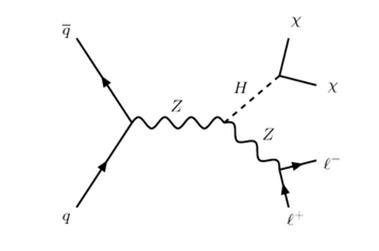
\includegraphics[scale=0.7]{HZ.png}
		\caption{Feynman diagram showing the associated production of a Higgs boson with a Z boson. The Higgs boson decays to two invisible DM particles and the Z boson decays leptonically, resulting in the $ll+ E_T^{miss}$ signature.}
		\label{fig:HZ}
	\end{center}
\end{figure}

The main Standard Model background processes for the $ll+$\met final state are \ZZ, $WZ\to lll\nu$, $WW\to l\nu l\nu$, $Z+$jets and $W+$jets. As discussed in Ref \cite{ZH_ATLAS}, the dominant source of background is the \ZZ process, contributing $\approx 60\%$ of the background. $WZ\to lll\nu$ events, where the $W$ boson decays into a electron or muon that escapes detection, account for 25\% of the total background. $Z(\to ll)+$jets process with misreconstructed \met contributes to about 8\% of the total background, and non-resonant-$ll$ processes, consisting of $t\bar{t}$, $Wt$, $WW$ and $Z\to\tau\tau$ production contribute similarly. $W+$jets, $VVV$, and $t\bar{t}V(V)$ backgrounds contribute to a minor extent ($<1\%$).

Figure \ref{fig:ZZ} shows the Standard Model production of $q\bar{q}\to ZZ$ and $gg\to ZZ$.

\begin{figure}[H]
	\begin{center}
		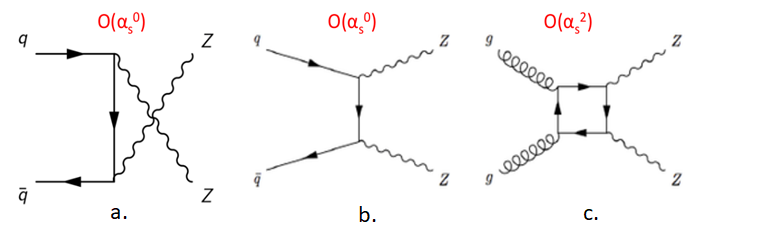
\includegraphics[scale=0.7]{ZZ.png}
		\caption{Feynman diagram showing $ZZ$ production, in the s-channel (a) and t-channel (b) induced by $q\bar{q}$, and induced by gluons (c).}
		\label{fig:ZZ}
	\end{center}
\end{figure}


\section{Transfer factor R}
To estimate the background, a transfer factor $R(p_T)$, it is defined to be the ratio of the cross sections of \ZZ to \Zg as a function of $p_T$, is introduced.
\begin{equation}
	R(p_{T}) = \frac{\sigma_{ZZ}(p_{T})}{\sigma_{Z\gamma}(p_T)}
\end{equation}
With the two processes being kinematically similar at high $p_T$, $R$ depends on the coupling of the $Z$ and $\gamma$ to quarks. It would be expected to reach a constant value at high $p_T$ that can be determined theoretically. In the following paragraph, an attempt is made to obtain a simple approximate calculation of $R$ from the contribution of $qq$ process.

The photon - quark and $Z$ boson - quark couplings in the Standard Model are given by,
\begin{equation}
	-ieQ_q\gamma^{\mu} \hspace{1 cm} \text{and} \hspace{1 cm}\frac{-ie}{2 \sin\theta_W \cos\theta_W}\gamma^{\mu}(v_q - a_q\gamma_5)
\end{equation}
respectively, where $Q_q,v_q$ and $a_q$ are respectively the electric, vector and axial neutral weak couplings of the quarks, and $\theta_W$ is the weak mixing angle. There is a contribution due to the $Z$ mass which appears in the internal propagators and phase space integration. This contribution becomes less important in the $p_T(\gamma)\gg M_Z$ region.

Thus, the leading order contributions from $q\bar{q}\rightarrow ZZ$ and $q\bar{q}\rightarrow Z\gamma$ are shown in Equation \ref{eq:theory_R}.
\begin{equation}
\begin{split}
	\sigma(q\bar{q}\rightarrow ZZ) &\propto \frac{1}{2}\frac{e^4\{(v_q^2 + a_q^2)^2 + 4v_q^2a_q^2\} }{16\sin^4\theta_W\cos^4\theta_W}\\[1.5ex]
	\sigma(q\bar{q}\rightarrow Z\gamma) &\propto \frac{e^2Q_q^2(v^2_q + a^2_q)}{4\sin^2\theta_W\cos\theta_W}
\end{split}
\label{eq:theory_R}
\end{equation}
The $u$ and $d$ quarks present in a $pp$ collision have different coupling strengths to the $Z$ boson as stated in Ref\cite{Z_coupling}, their relative contributions are accounted for using Equation \ref{eq:u_d_contrib}
\begin{equation}
R = \frac{\sigma(u\bar{u}\rightarrow ZZ)\langle u\rangle + \sigma(d\bar{d}\rightarrow ZZ)\langle d\rangle}{\sigma(u\bar{u}\rightarrow Z\gamma)\langle u\rangle + \sigma(d\bar{d}\rightarrow Z\gamma)\langle d\rangle}
\label{eq:u_d_contrib}
\end{equation}
Using the vector and axial couplings of the $Z$ boson to $u$ and $d$ quarks\footnote{Vector and Axial couplings of Z to $u$ and $d$ quarks: $v_u = 0.18, a_u = 0.50, v_d = -0.35, a_d = -0.514$}, assuming $\langle d \rangle/\langle u\rangle = 0.5$ and setting $\sin^2\theta_W = 0.2315$, $R\approx 1.28$ for the dominant $q\bar{q}$ interaction.
%\section{Theoretical aspects}
%
%The Standard Model is based on the formalism of quantum field theories (QFTs), in which particles are intepreted as excitations of underlying fields.
%
%\subsection{Quantum Electrodynamics}
%Quantum Electrodynamics (QED) is the relativistic quantum field theory of electromagnetism. It encompasses all particles having a charge (which includes all the quarks and charged leptons, and their charged composite particles), and the photon as the mediator of interactions between these.
%
%Quantum Electrodynamics is extended to describe the electroweak theory, which includes neutrinos, and the $W$ and $Z$ bosons as mediators of interactions.
%
%\subsection{Quantum Chromodynamics}
%Quantum Chromodynamics (QCD) is the quantum field theory of strong interactions. It describes particles that have color charge (such as quarks, and their composite particles),and is mediated by gluons.
%
%QCD has some interesting properties. For example, the force between two color charges remains constant, a phenomenon known as $color\ confinement$. Thus, separating quarks requiring increasing amounts of energy. Eventually it becomes energetically favorable to simple create a quark-antiquark pair from vacuum, forming color neutral hadrons. Another interesting property is that the strength of quark-gluon interactions decreases as the energy scale of the interaction increases (equivalently, the length scale of the interaction decreases). This phenomenon is known as asymptotic freedom; essentially, quarks and gluons in close proximity behave as nearly free particles, while those far apart interact strongly.
%
%While there is no analytic proof of QCD, there is a large body of evidence supporting its predictions.
%
%\subsection{Feynman diagrams}
%Feynman diagrams are a powerful tool in calculating the likelihood of interactions between fundamental particles. Not only are they an intuitive diagrammatic representation of processes, but they can also be directly translated into an equation that can be integrated to give the transition amplitude between the initial and final state in a process.
%
%The rules that provide the convention for this translation are called Feynman rules. They are motivated by the quantum field theoretical formulation of the Standard Model, but what makes these diagrams so powerful is that once the rules are laid down, knowledge of QFT is not required. The derivation of the same equations from QFT can be very involved and messy, and Feynman diagrams are a clear and concise packaging of the same.
%\begin{figure}[H]
%\centering
%	\begin{subfigure}{0.4\textwidth}
%	\centering
%		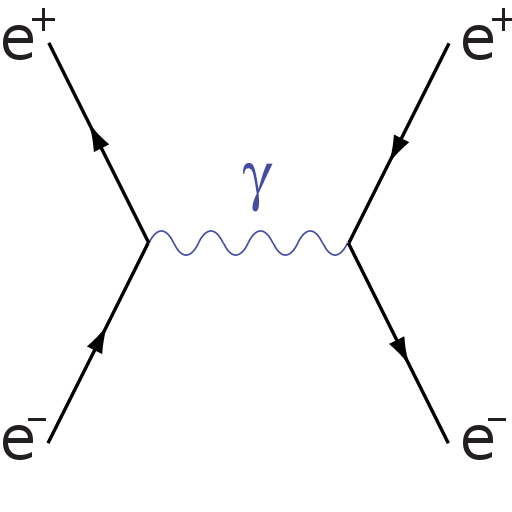
\includegraphics[width=0.5\linewidth]{Bhabha_S_channel.png}
%	\end{subfigure}
%	\begin{subfigure}{0.4\textwidth}
%	\centering
%		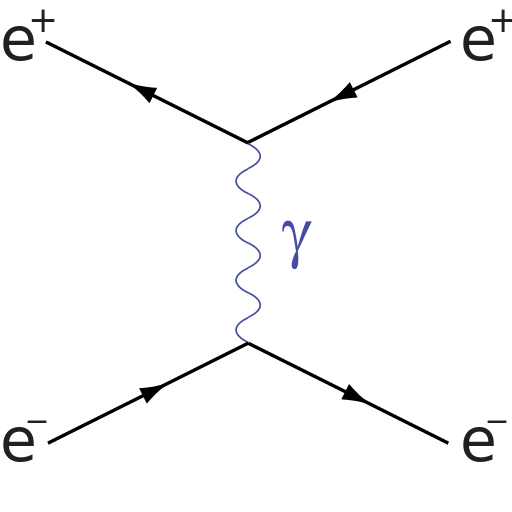
\includegraphics[width=0.5\linewidth]{Bhabha_T_channel.png}
%	\end{subfigure}
%	\caption{Bhabha scattering showing electron-positron annihilation in s-channel (left) and scattering in t-channel (right). The interaction is mediated by the photon, the gauge boson that mediates electromagnetic interactions}.
%	\label{fig:bhabha}
%\end{figure}
%Figure \ref{fig:bhabha} shows Bhabha scattering, an electromagnetic process involving the interaction of an electron and a positron, mediated by a photon. The Feynman rules assign functionals to the propagators (the straight/wavy lines in the diagram) and the vertices, from which we can obtain the amplitudes for this process.

\chapter{Theoretical uncertainties on cross sections and the transfer factor R}

It is worth reiterating that the goal of this thesis is to use \Zg process to estimate the dominant contribution \ZZ to the Standard Model \llM background. Excesses would indicate the presence of BSM physics. It is thus important to have an estimate of the uncertainties on the theoretical predictions of the $ZZ$ and $Z\gamma$ cross sections, and the transfer factor $R$.\\
In this study, the following sources of uncertainities are studied.
\begin{itemize}
\item Scale Uncertainties: contributions due to higher order QCD corrections cannot be calculated to arbitrarily high order, as it gets progressively more computationally expensive. Thus, this study is limited to Next to Leading Order (NLO), and further corrections are accounted for as scale uncertainties.
\item PDF Uncertainties: a proton-proton collision involves the interaction of the composite quarks and gluons (partons) at very high energies. These partons carry a fraction of the proton momentum. Parton Distribution Functions (PDFs) represent this fraction of proton momentum carried by partons as probability distributions. Owing to the non-deterministic nature of this fact, this study attempts to account for this uncertainties as PDF uncertainties.
\item Photon Fragmentation Uncertainties: in the \Zg process, the signal includes a photon. However, while reconstructing the event, soft photons, or photons resulting from other fragmentation processes may be encountered. To ensure that the photon is indeed prompt, it is required to be isolated from hadronic activity (such as pion decays). This isolation is implemented experimentally in different ways. The uncertainty associated with the implementation of this isolation is estimated as photon fragmentation uncertainties.
\end{itemize}

To characterize these uncertainties, we use a programme, MCFM, to generate cross sections for \ZZ and \Zg processes, and vary the relevant parameters such as scale, PDF sets, and photon isolation effects to obtain an estimate of the uncertainties.

\newpage
\section{MCFM}
MCFM is a program that calculates cross sections for femtobarn-level processes at LO or NLO. In this study, MCFM v8.0 \cite{MCFM} is used to produce cross sections of \ZZ and \Zg processes at NLO, with a selection of generator level cuts. The generation parameters in MCFM allow fine control over the sample, such as PDF sets, photon isolation, lepton and photon $p_T$ and $\eta$, renormalization and factorization scales, etc. The samples are generated with cuts on $E_T^{miss} = p_T(Z\to \nu\nu)$ for the $ZZ$ process and $p_T(\gamma)$ for the $Z+\gamma$ process. A ratio of these cross sections is taken to obtain the $R$ distribution as a function of $p_T$. The uncertainty on $R$ is calculated by varying several parameters at the generator level, such as the renormalization and factorization scales, the PDF sets used, photon fragmentation, etc. The contributions of the $q \bar{q}$ and $gg$ processes are estimated separately.

In MCFM generated events containing a leptonically decaying $Z$ boson, $Z\rightarrow ee$ only i.e. the decay is constrained to just one flavor, electrons. As electrons and muons have similar properties with the exception of mass, simply the branching fraction of $Z\rightarrow ee$ must be accounted for to obtain the inclusive value of $R$.
\begin{equation}\label{eq:R_inc}
	R_{inc} = R * \frac{BR(Z\rightarrow ee)}{BR(Z \rightarrow ee)*BR(Z\rightarrow \nu\nu)*2}
\end{equation}

\noindent\textbf{Note : Unsure how to expand this section}
\section{Generator Parameters}
The samples are generated using MCFM v8.0.
\renewcommand{\thefootnote}{\fnsymbol{footnote}} 
Table \ref{table:default} lists the generator level settings used for the $ZZ$ and $Z+\gamma$ processes. All lepton cuts are consistent with the ones used in the ATLAS Z+$E_T^{miss}$ analysis \cite{ZH_ATLAS}.
\begin{table}[H]
\begin{center}
	\begin{tabular}{|c|c|c|}
	\hline
	\textbf{Cuts} &$ZZ \rightarrow ee\nu\nu$ & $Z(\rightarrow ee)+\gamma$\\
	\hline
	Process ID & 87 & 300\\
	$M_{ee}$ & $76 < M_{ee} < 106$ GeV & $76 < M_{ee} < 106$ GeV\\
	$M_{\nu\nu}$ & - & -\\
	Order & NLO & NLO\\
	PDF set & CT14 & CT14\\
	$p_T^{\text{lead}}(e)$ & $> 30$ GeV & $> 30$ GeV\\
	$|\eta^{lead}(e)|$ & $< 2.47$ & $< 2.47$\\
	$p_T^{\text{sublead}}(e)$ & $> 20$ GeV & $> 20$ GeV\\
	$|\eta^{sublead}(e)|$ & $< 2.47$ & $< 2.47$\\
	$p_T(V)$\footnotemark & $> 90$ GeV & $> 90$ GeV\\
	Renormalization scale & $H_T = \sum_i p_{T,i}$& $H_T = \sum_i p_{T,i}$\\
	Factorization scale & $H_T = \sum_i p_{T,i}$& $H_T = \sum_i p_{T,i}$\\
	\hline
	\end{tabular}
	\caption{Settings in input.DAT for MCFM}
	\label{table:default}
	\end{center}
\end{table}
\footnotetext{$V$ is a vector boson: $Z(\to\nu\nu)$ for the $ZZ$ process; $\gamma$ for the $Z\gamma$ process}
\renewcommand{\thefootnote}{\arabic{footnote}}
The constraint on $M_{ee}$ in the case of $Z+\gamma$ suppresses the FSR process by ensuring that the lepton pair are from a $Z$ decay only.
\newpage
\section{Results}
Using the settings listed in Table \ref{table:default}, the cross sections for $ZZ\to ee\nu\nu$ and $Z\gamma\to ee\gamma$ are generated, as shown in Figure \ref{xsecs}. Throughout this analysis, these samples are the reference.
\begin{figure}[H]
\centering
	\begin{subfigure}{0.49\textwidth}
		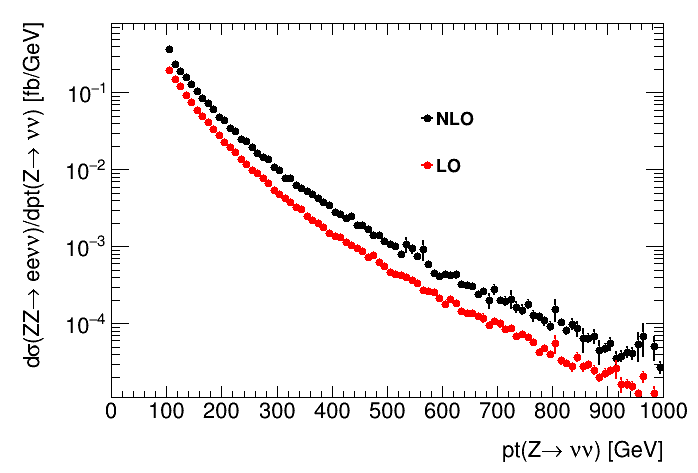
\includegraphics[width=\linewidth]{ZZ_xsec.png}
		\caption{}
		\label{subfig:ZeeZvv}
	\end{subfigure}	
	\begin{subfigure}{0.49\textwidth}
		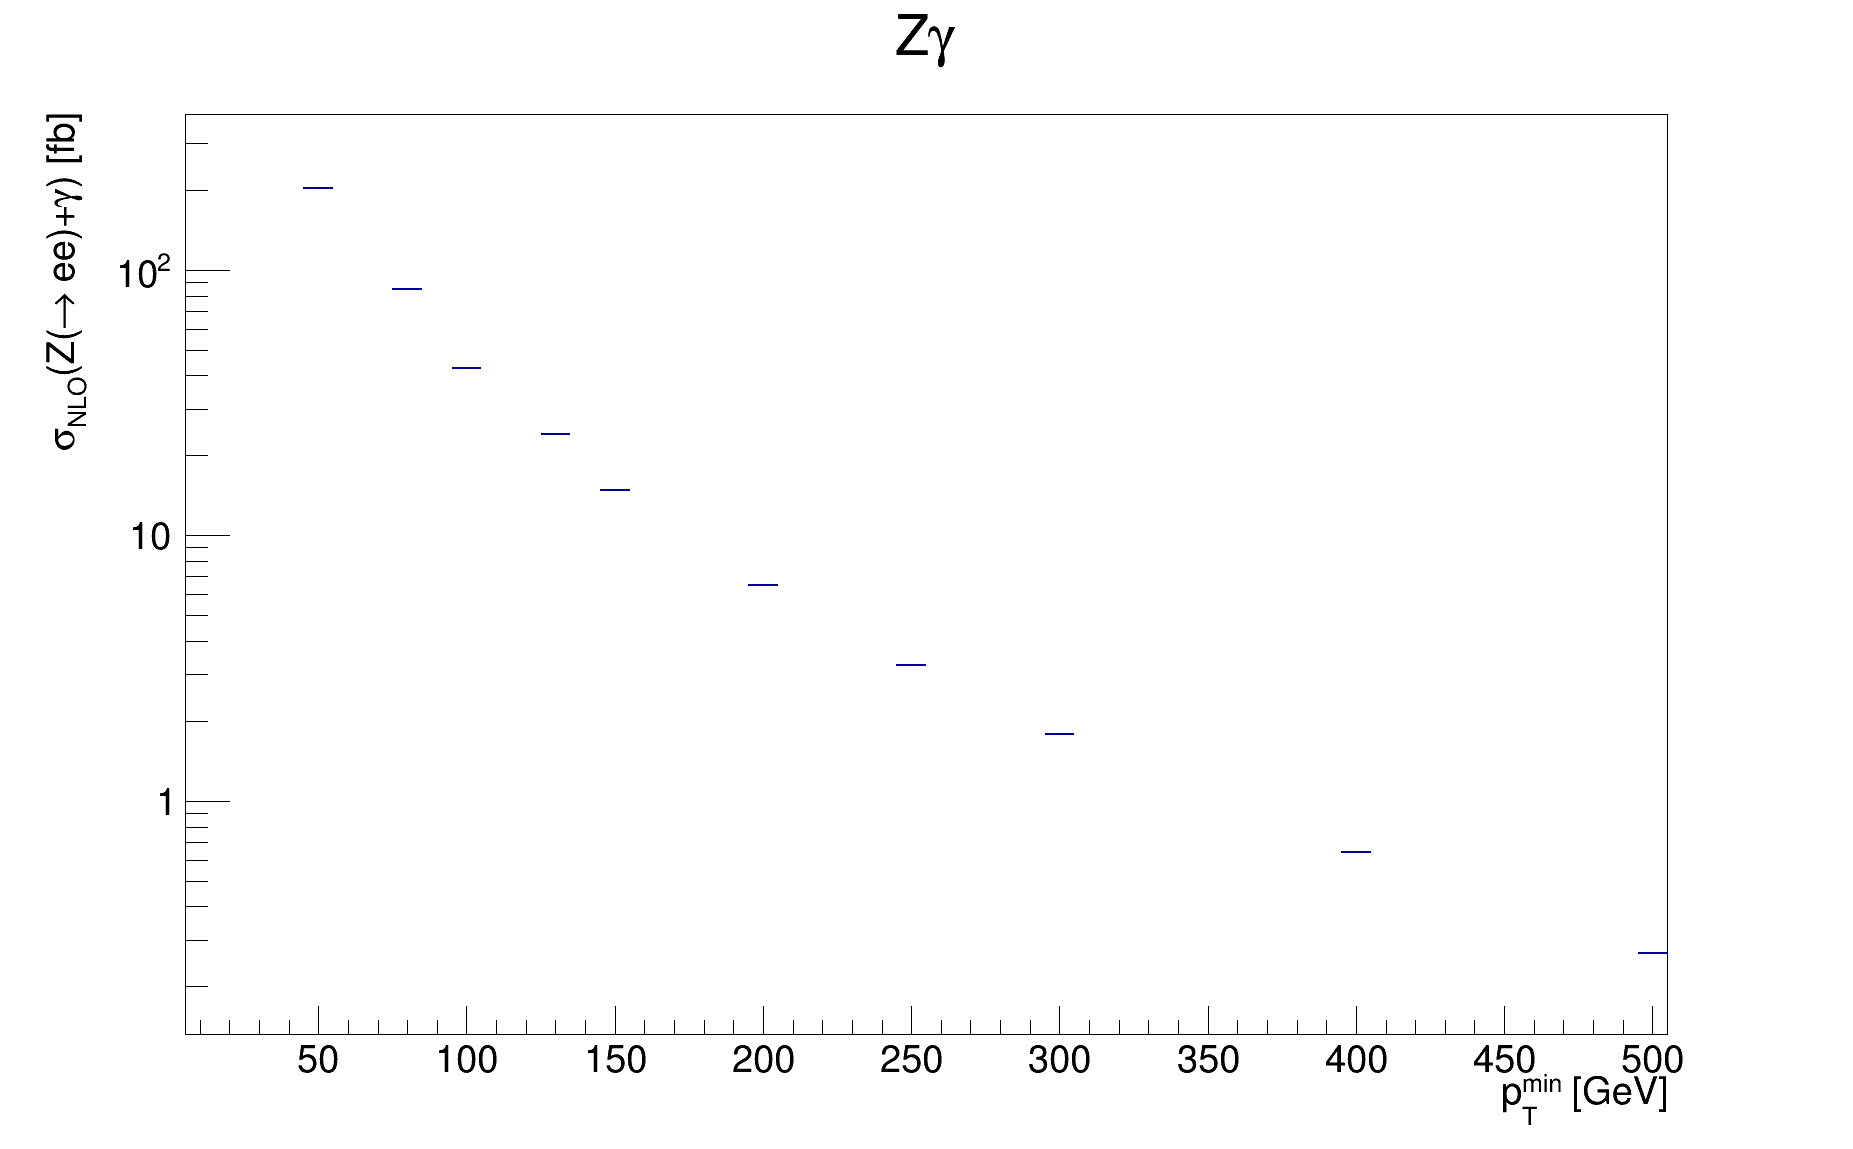
\includegraphics[width=\linewidth]{Zg_xsec.png}
		\caption{}
		\label{subfig:Zeeg}	
	\end{subfigure}
	\caption{NLO and LO cross sections of $ZZ\to ee\nu\nu$ (left) and $Z\gamma\to ee\gamma$ (right) processes with the cuts as in Table 1. The vertical axis is in $\log_{10}$ scale. The leptonically decaying $Z$ boson decays to an $e^+e^-$ pair. There is no flavor constraint on the neutrinos.}
	\label{xsecs}
\end{figure}
The ratio $R = \sigma(ZZ\rightarrow ee\nu\nu)/\sigma(Z\gamma\rightarrow ee\gamma)$ is shown in Figure \ref{fig:Rcurve}, taken as the ratio of the cross sections in Figures \ref{subfig:ZeeZvv} and \ref{subfig:Zeeg}. Additional events are generated with \met and $p_T(\gamma) > 400$ GeV for the two processes respectively to increase statistics. 
\begin{figure}[H]
	\centering
	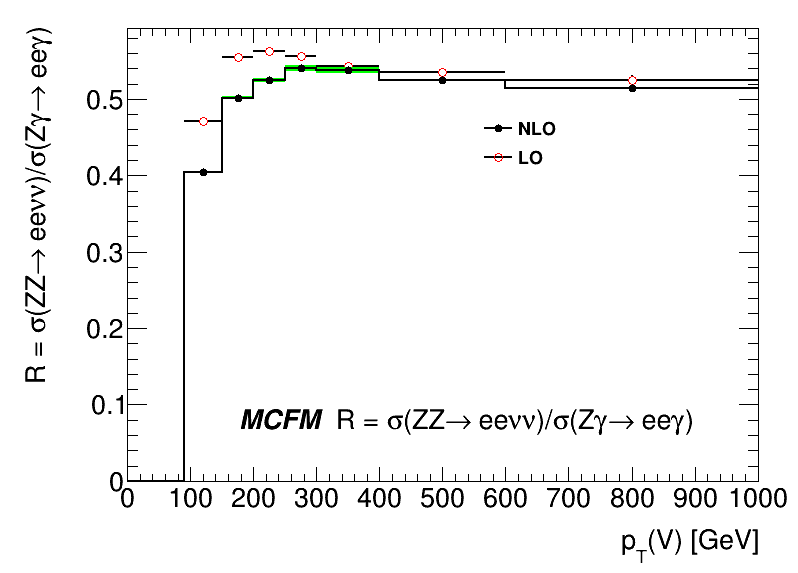
\includegraphics[width= 0.7\textwidth]{R.png}
	\caption{The transfer factor $R$ as a function of $p_T$, taken as a ratio of  the $ZZ\to ee\nu\nu$ and $Z\gamma\to ee\gamma$ cross sections at both LO and NLO. The leptonically decaying $Z$ boson decays to an $e^+e^-$ pair.}
	\label{fig:Rcurve}
\end{figure}
The $R$ value is observed to increase from $\approx 0.39$ at 50 GeV to $\approx 0.52$ at high $p_T$, where it reaches a plateau. When the branching ratio of $Z$ boson decaying selectively to $e^+e^-$, or to $\nu\nu$, is accounted for as shown in Equation \ref{eq:R_inc}, the resulting ratio $R(p_T)$ is shown in Figure \ref{fig:RcurveBR}, which shows the ratio of $\sigma(ZZ)$ to $\sigma(Z\gamma)$, i.e. if the $Z$ bosons do not decay further. The value of $R$ is observed to increase from $\approx 0.98$ at 50 GeV to $\approx 1.3$ at high $p_T$, in reasonable agreement with the simple approximate calculation presented in Chapter \ref{ch:theory} of $R \approx 1.28$.
\begin{figure}[H]
	\centering
	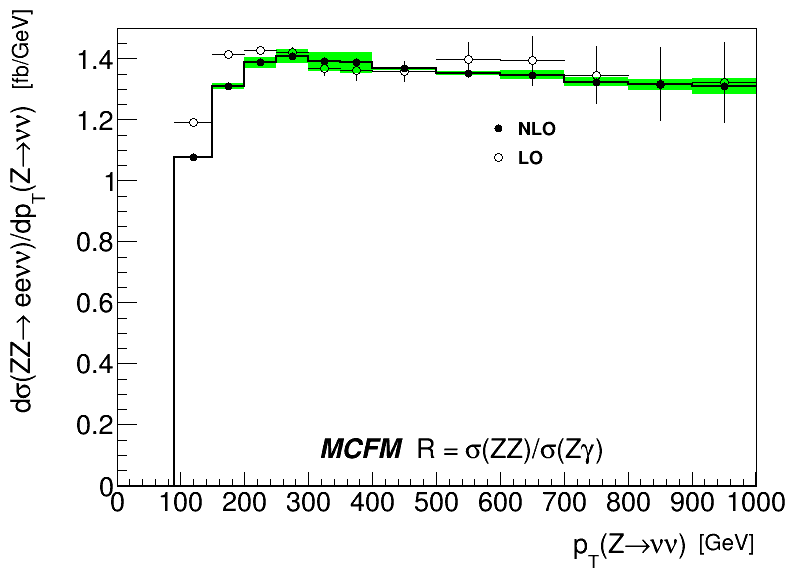
\includegraphics[width = 0.7\textwidth]{R_BR.png}
	\caption{The transfer factor $R$ as a function of $p_T$ at both LO and NLO, adjusted for the $Z\rightarrow ee$ and $Z\rightarrow \nu\nu$ branching ratios. This shows the $R=\sigma(ZZ)/\sigma(Z\gamma)$, where the $Z$ bosons do not decay.}
	\label{fig:RcurveBR}
\end{figure}
\textbf{Note : Need to flesh out the captions for the next few plots}

Figure\ref{fig:yy} shows the normalized rapidity distributions for missing transverse momentum $(Z\to\nu\nu)$ and the photon respectively.
\begin{figure}[H]
\centering
	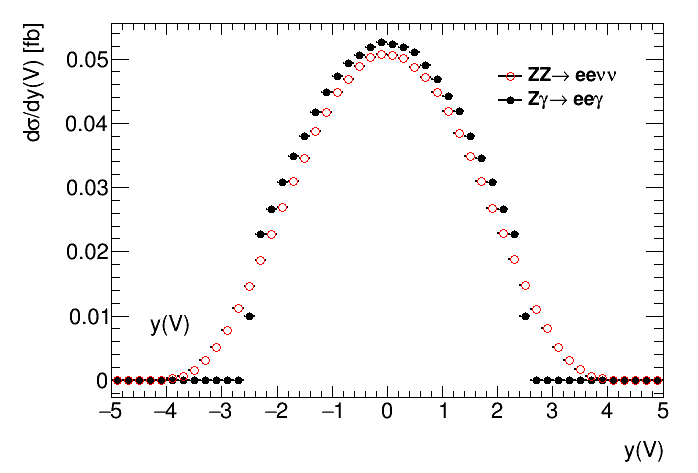
\includegraphics[width=0.7\textwidth]{yy.png}
	\caption{y(V)}
	\label{fig:yy}
\end{figure}
Figures \ref{fig:leppt} and \ref{fig:leptony} further illustrate the topology of the events by showing normalized distributions for the leading and subleading lepton $p_T$ and rapidity.
\begin{figure}[H]
\centering
	\begin{subfigure}{0.49\textwidth}
		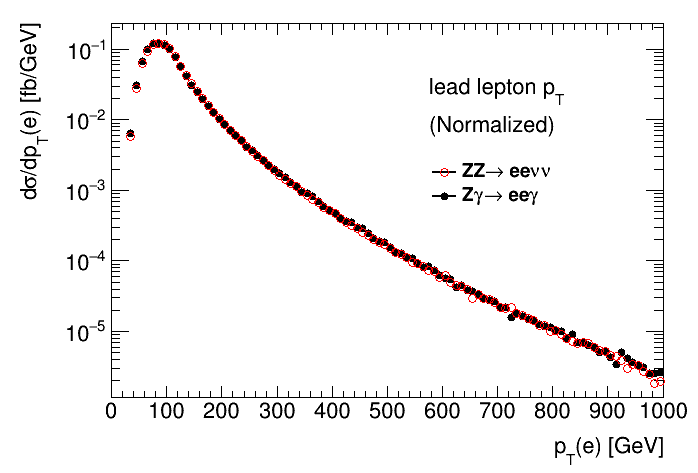
\includegraphics[width=\linewidth]{leadpt.png}
		\caption{}
		\label{fig:leadpt}
	\end{subfigure}
	\begin{subfigure}{0.49\textwidth}
		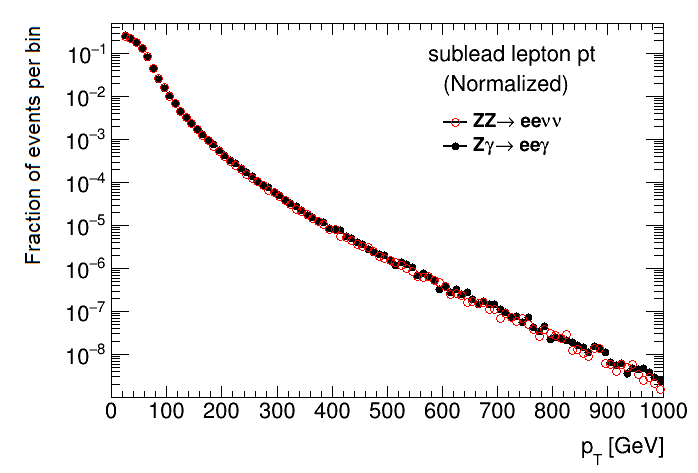
\includegraphics[width=\linewidth]{subleadpt.png}
		\caption{}
		\label{fig:subleadpt}
	\end{subfigure}
	\caption{Normalized distributions showing the transverse momentum of the leading (left) and subleading (right) leptons for the two processes.}
	\label{fig:leppt}
\end{figure}
\begin{figure}[h]
\centering
	\begin{subfigure}{0.49\textwidth}
		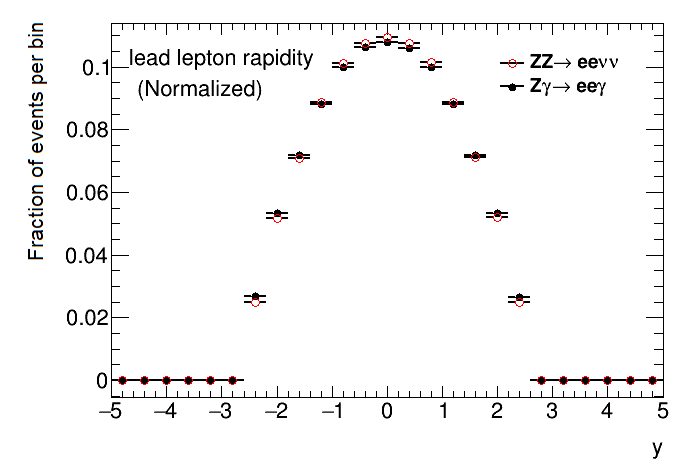
\includegraphics[width=\linewidth]{leady.png}
		\caption{}
		\label{fig:leady}
	\end{subfigure}
	\begin{subfigure}{0.49\textwidth}
		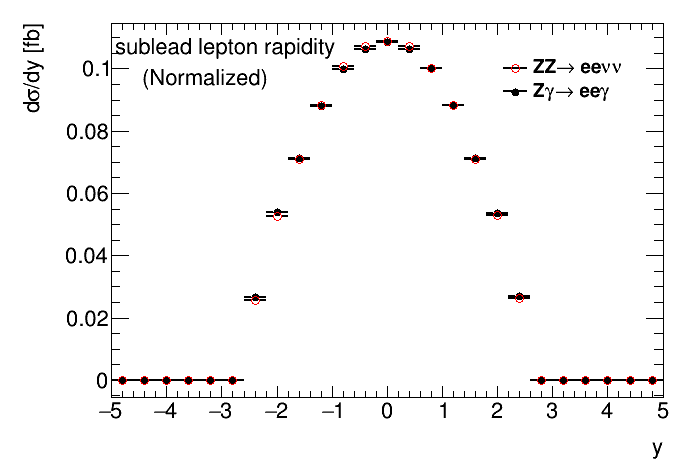
\includegraphics[width=\linewidth]{subleady.png}
		\caption{}
		\label{fig:subleady}
	\end{subfigure}
	\caption{Normalized distributions showing the transverse momentum of the leading (left) and subleading (right) leptons for the two processes.}
	\label{fig:leptony}
\end{figure}

Gluon-gluon processes contribute to 8.6\% of the total cross section for the $ZZ$ process and 2.5\% of the $Z+\gamma$ process. Figure \ref{fig:xsec_gg_qq} shows the $ZZ$ and $Z\gamma$ cross sections ($Z$ boson decay constrained to only $e^-e^+$ and $\nu\bar{\nu}$ only) from the contributing $q\bar{q}$, $qg$ and $gg$ subprocesses.
\begin{figure}[H]
\centering
	\begin{subfigure}{0.49\textwidth}
		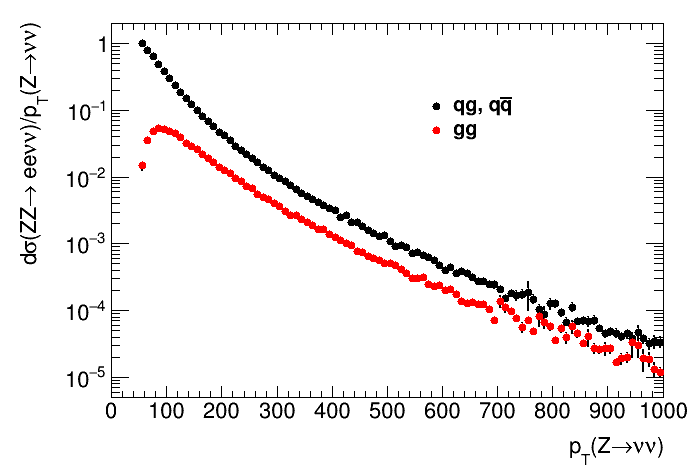
\includegraphics[width=\linewidth]{ZZ_subproc.png}
	\end{subfigure}
	\begin{subfigure}{0.49\textwidth}
		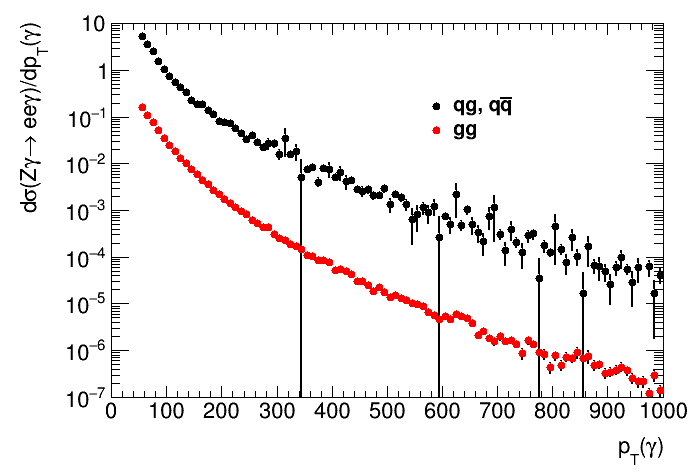
\includegraphics[width=\linewidth]{Zg_subproc.png}
	\end{subfigure}	
\caption{The cross sections of $ZZ\to ee\nu\nu$ (left) and $Z\gamma\to ee\gamma$ (right) as a function of $p_T$, from the contributing $q\bar{q}$, $qg$ and $gg$ processes. The leptonically decaying $Z$ boson decays to an electron-positron pair}
\label{fig:xsec_gg_qq}
\end{figure}
The $R_{gg}$ distribution, shown in Figure \ref{fig:R_ggonly} is observed to approach an asymptotic value at a much higher $p_T = 1.5$ TeV. The shape and scale of the $R_{gg}$ distribution remain to be understood, as they differ from Figure \ref{fig:Rcurve}.
\begin{figure}[H]
\centering
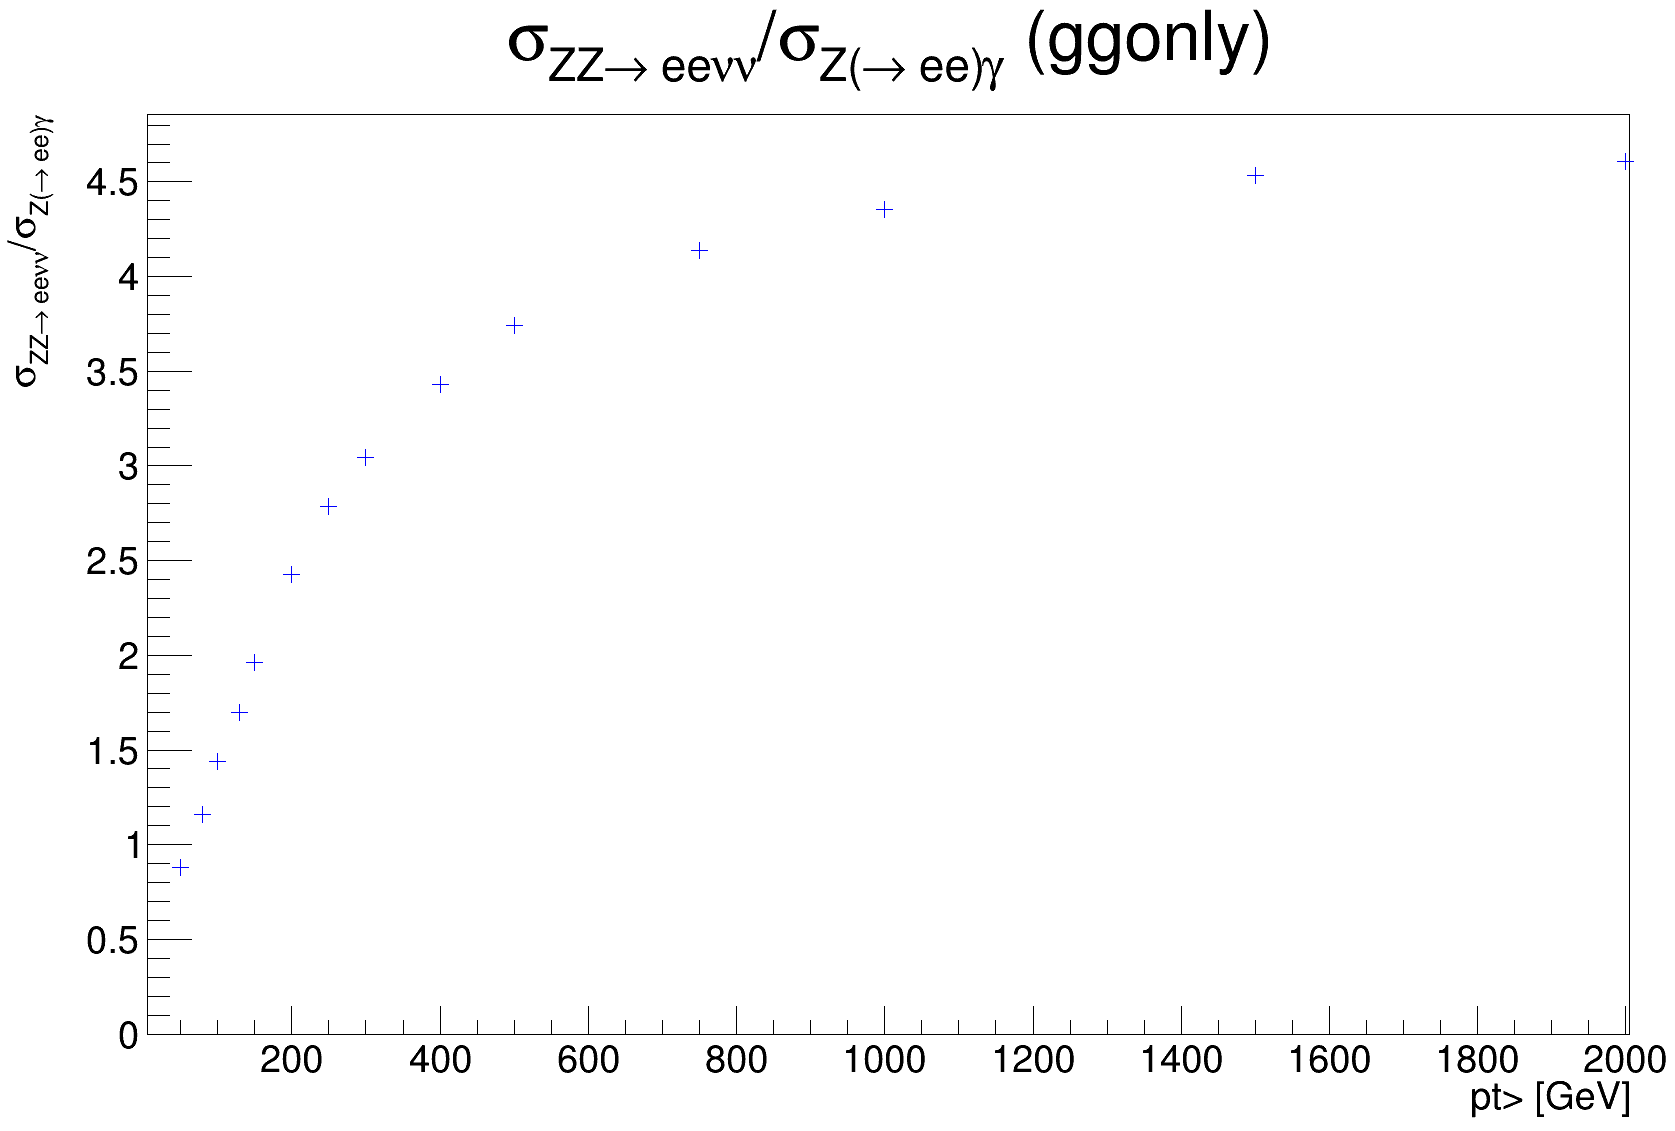
\includegraphics[width=0.7\textwidth]{R_ggonly.png}
\caption{$R_{gg}(p_T)$, computed from the contributions of the $gg$ subprocess to the cross sections of $ZZ$ and $Z\gamma$. The curve reaches a plateau at a much higher $p_T$ than for contributions from the $q\bar{q}$ process only.}
\label{fig:R_ggonly}
\end{figure}

\subsection{Uncertainty from Scale Variation}
In higher order QCD calculations, perturbative corrections may be added to the vertices or propagators in a Feynman diagram. Physically, these corrections occur at very small time scales. These loop integrals that correspond to these corrections diverge. The higher the order, the more difficult the calculation is. It is possible to introduce an arbitrary cut-off scale $\mu$ such that up to a given order, the effect of these corrections can be absorbed into the strong coupling constant $\alpha_s(\mu)$.

Two kinds of divergences are encountered: infrared divergences, and ultraviolet divergences. Infrared divergences occur for an on-shell internal propagator, and ultraviolet divergences are logarithmic divergences that occur as the integration variable approaches $\infty$. They correspond to physics at long and short distances\footnote{Long distances are those where soft interactions take place, away from the hard parton-parton interaction. Short distances are those where the hard parton parton interactions occur.}, respectively. The infrared divergences are addressed by the inclusion of the factorization scale $\mu_F$, while the ultraviolet divergences are addressed by the inclusion of the renormalization scale $\mu_R$. These parameters are arbitrary, and are set by hand. These are then varied between $\frac{1}{2}\mu < \mu < \ 2\mu$ to obtain an indication of the dependence of the matrix element on the scales, and thus, the uncertainty around the chosen scale. 

To address scale uncertainties in this study, the prescription used in Ref \cite{precise_scale}, section 4 is followed. The central scale, $\mu_0$ is chosen to be $H_{T}/2$ for both \ZZ and \Zg samples (where $H_T$ is the scalar sum of the transverse momentum of all particles after collision, $\sum_{i} p_{T,i}$), and seven-point variations are applied, i.e.
\begin{equation}
\frac{\mu_i}{\mu_0} = (1,1),(1,2),(2,1),(2,2),(0.5,1),(1,0.5),(0.5,0.5)\\
\label{eq:scale}
\end{equation}
where $i=0,...,6$. The central cross section value is taken to be the mean of the maximum and minimum cross sections resulting from this variation, and the uncertainty to be the half the difference between the same.
\begin{align}
\sigma_{NLO}^{(V)} &= \frac{1}{2}\left[\sigma_{NLO}^{(V,max)} + \sigma_{NLO}^{(V,min)}\right]\label{eq:scale_central}\\
\delta\sigma_{NLO}^{(V)} &= \frac{1}{2}\left[\sigma_{NLO}^{(V,max)} - \sigma_{NLO}^{(V,min)}\right]
\label{eq:scale_central2}
\end{align}
where
\begin{align}
\sigma_{NLO}^{(V,max)} &= max\left\lbrace\sigma_{NLO}^{(V)}(p_{T}(V),\mu_i)|0\leq i \leq 6\right\rbrace\\
\sigma_{NLO}^{(V,min)} &= min\left\lbrace\sigma_{NLO}^{(V)}(p_{T}(V),\mu_i)|0\leq i \leq 6\right\rbrace
\end{align}
and $V = Z\to\nu\nu$ for \ZZ, or $V = \gamma$ for \Zg. This uncertainty is propagated to $R$.

To estimate the degree of correlation between the processes, the process dependent part of the cross sections may be used. The highest available term in the perturbative expansion is considered to define a $K$-factor. Since the study is undertaken at NLO, the $K$-factor is defined as in Equation \ref{eq:K_factor}.
\begin{equation}
K_{NLO}^{(V)} = \sigma_{NLO}^{(V)}(p_T)/\sigma_{LO}^{(V)}(p_T)
\label{eq:K_factor}
\end{equation}

To estimate the unknown process dependent correlation effects, the difference between the $K$-factors of the \ZZ and \Zg processes is taken.
\begin{equation}
\delta^{(2)} \sigma_{NLO} = K_{NLO}^{(\gamma)}(p_T) - K_{NLO}^{(Z)}(p_T)
\label{eq:K_factor_unc}
\end{equation}

Applying the above prescription, the variation of scales for cross sections of $ZZ\to ee\nu\nu$ and $Z\gamma\to ee\gamma$ are shown in Figure \ref{fig:scale_xsec} below.
\begin{figure}[H]
\centering
	\begin{subfigure}{0.49\textwidth}
		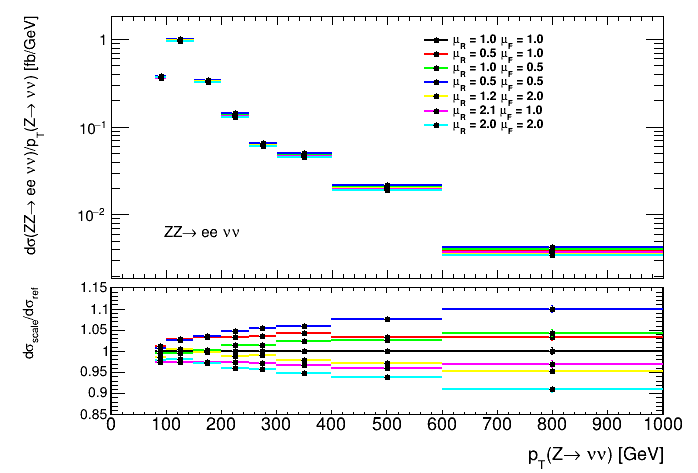
\includegraphics[width=\linewidth]{zz_scale.png}
	\end{subfigure}
	\begin{subfigure}{0.49\textwidth}
		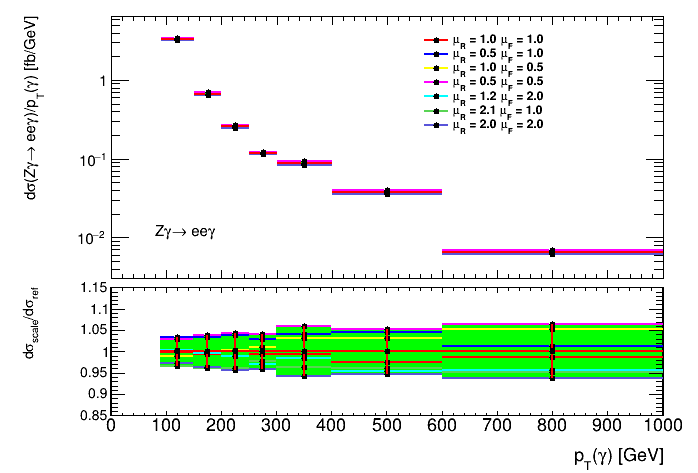
\includegraphics[width=\linewidth]{zg_scale.png}
	\end{subfigure}
	\caption{The scale variations around the cross sections of $ZZ\to ee\nu\nu$(left) and $Z\gamma\to ee\gamma$(right)}
	\label{fig:scale_xsec}
\end{figure}

At 100 GeV, the deviation from the central value is about 3\% for both processes and increases to ~10\% at high $p_T$. Here, the prescription in Equations \ref{eq:scale_central} and \ref{eq:scale_central2} is used to compute the central value and uncertainty.\\ Treating the scales as correlated between the processes, the scale variation for the transfer factor $R$ is shown in Figure \ref{fig:R_scale}. The central value of $R$ and the uncertainty band around it is taken according to Equations \ref{eq:scale_central} and \ref{eq:scale_central2} applied to $R$.
\begin{figure}[H]
\centering
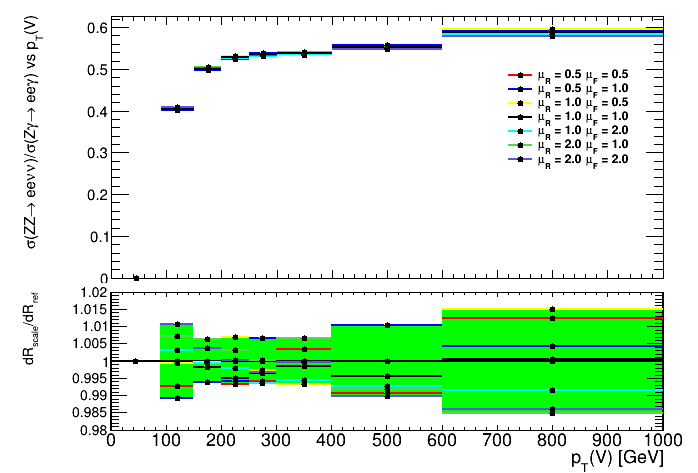
\includegraphics[width=0.7\textwidth]{R_scale.png}
\caption{The transfer factor $R = \sigma(ZZ\to ee\nu\nu)/\sigma(Z\gamma\to ee\gamma)$(top), with the scales varied in a correlated manner for both $ZZ$ and $Z\gamma$ processes. The bottom plot shows the relative ratio $R_i/R_0$ of the varied transfer factors to the central value.}
\label{fig:R_scale}
\end{figure}
The correlated scale uncertainty around $R$ is lower compared to that of the individual cross sections. At 100 GeV, $R \approx 0.4 \pm 0.037$, or an uncertainty of 1\%. At high $p_T$, $R\approx 0.55 \pm 0.01$, the uncertainty is 1.8\%.

To study the uncertainty due to unknown process dependent correlation effects, the $K$-factor study is undertaken, following the prescription in Equations \ref{eq:K_factor} and \ref{eq:K_factor_unc}. Figure \ref{fig:K_pt}
\begin{figure}[H]
\centering
	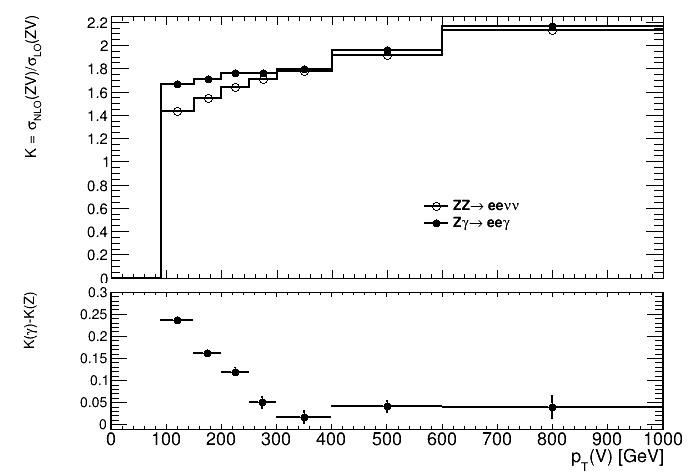
\includegraphics[width=0.7\textwidth]{K_pt.png}
	\caption{The $K$ factor to estimate the unknown process dependent correlations, defined as $\sigma_{NLO}(V)/\sigma_{LO}(V)$. The bottom plot shows the $K$-factor difference relative to $K(Z)$.}
	\label{fig:K_pt}
\end{figure}

\textbf{Note : Work in progress with the last bin}.

\subsection{Uncertainty from PDF variation}
A proton is a Baryon, i.e. it is composed of 3 quarks and several gluons. In a proton-proton collision, it is these quarks and gluons, called $partons$ that actually interact. This is illustrated by Figures $the\ feynman\ diagrams\ in\ Chapter\ 3$, which show the Feynman diagrams for quark-quark and gluon-gluon interactions. Thus it is important to know the momentum of the interacting partons. It is not possible to deterministically know the momentum of the partons, as it is the momentum of the protons that is set during the experiment. However, the fraction of the proton momentum that is carried by the partons can be modelled as probability distributions.

Parton Distribution Functions (PDFs) characterize the fraction of proton momentum carried by partons as probability distributions. PDF sets are collections of PDFs that model the uncertainty associated with parton momenta. The PDF set used for reference is the \texttt{CT14}\cite{CT14} PDF set. The uncertainty on the PDFs is studied by using the 30 variations provided by the \texttt{PDF4LHC15} set\cite{PDF4}, constructed from the combination of \texttt{CT14,MMHT14}\cite{MMHT14} and \texttt{NNPDF3.0}\cite{NNPDF3} PDF sets. These sets are provided by LHAPDF6\cite{LHAPDF}. \texttt{PDF4LHC15} provides a set of variations that include those determined by different groups (MSTW, CTEQ and NNPDF). The set used here is \texttt{PDF4LHC15\_nlo\_30}, consisting of 30 members. While the most accurate uncertainties are given by \texttt{PDF4LHC15\_nlo\_100} set, \texttt{PDF4LHC15\_nlo\_30} is used here for a faster, reasonably accurate estimate of the uncertainties.
\begin{figure}[H]
\centering
	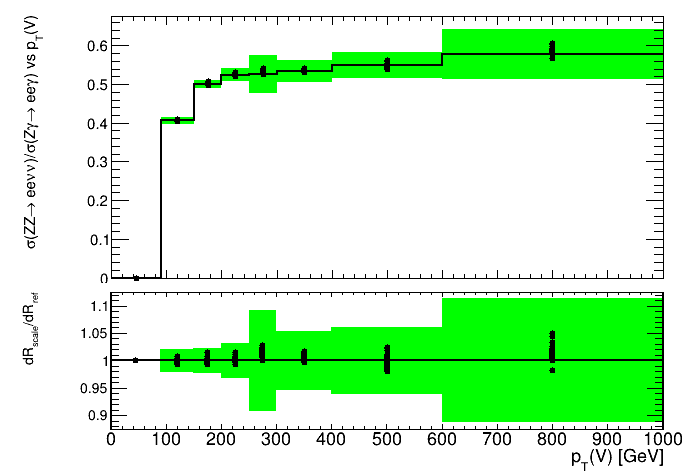
\includegraphics[width = 0.7\textwidth]{R_pdf.png}
	\caption{The transfer factor $R = \sigma(ZZ)/\sigma(Z\gamma)$ (top), and the relative ratio $R_i/R_0$ of the transfer factor  calculated using PDF sets 1-30, with respect to set 0 which is taken as the central value. }
	\label{fig:PDF30var}
\end{figure}
\noindent Fig.\ref{fig:PDF30var} shows the comparison of the ratio $R(p_T)$ from the 30 member sets of \texttt{PDF4LHC15\_nlo\_30}. To measure the uncertainty due to these 30 sets, analogous to Equation 20 in Ref \cite{PDF4}, Equation \ref{eq:PDFerr} is used:
\begin{equation}\label{eq:PDFerr}
	\delta^{PDF}R = \sqrt{\sum^{N_{mem}}_{k=1} (R^{(k)} - R^{(0)})^2}
\end{equation}
where $N_{mem}$ is the number of member sets in the group, in this case, 30.

\textbf{Note : Still trying to figure out why the uncertainty is so large in the continuous distribution as opposed to the discrete data point run we did initially. Investigating statistical error by generating more high pt events.}

\noindent The combined uncertainty around $R \approx 0.40$ is $\pm 0.008$, or about 2\%, at 100 GeV. The uncertainty is significantly larger at high $p_T$ values, $>10\%$.

\subsection{Uncertainty from Photon Fragmentation}
The \Zg process may contain photons that arise from the hadron showers. It is therefore important to isolate the prompt photon from hadronic activity. This reduces unwanted background from pion decays, or fragmentation processes.

Experimentally, photon isolation is implemented with the following cuts:
\begin{equation}
\sum_{\in R_0} E_T(\text{had}) < \epsilon_h p_T^\gamma \text{\hspace{1cm} or \hspace{1cm}} \sum_{\in R_0} E_T(\text{had}) < E_T^{max}
\end{equation}
\label{eq:photon_isol}
limiting the transverse hadronic energy $E_T(had)$ in a cone of size $R_0 = \sqrt{\Delta\eta^2 + \Delta\phi^2}$ around the photon, to some fraction of the photon $p_T$, or some fixed small cut-off.

The smooth cone isolation method of Frixione \cite{frixione} is an alternative isolation procedure, which simplifies calculations by avoiding fragmentation contribuitions. The following isolation prescription is applied to the photon:
\begin{equation}
	\sum_{R_{j\gamma} \in R_0} E_T(\text{had}) < \epsilon_h p_T^\gamma \left(\frac{1-\cos R_{j\gamma}}{1-\cos R_0}\right)^n.
\end{equation}
\label{eq:frix_isol}
where $R_{j\gamma}$ is the separation of the photon and the $j^{th}$ hadron. This requirement constrains the sum of hadronic energy inside a cone of radius $R_{j\gamma}$, for all separations $R_{j\gamma}$ less than a chosen cone size $R_0$. This prescription allows soft radiation inside the photon cone, but collinear singularities are removed. The smooth cone isolation is infrared finite, thus fragmentation contributions do not need to be included.\\
The relative isolation, given by Equation \ref{eq:photon_isol} is used in experimental analyses, while smooth isolation is difficult to implement experimentally. However, comparing both methods gives us an estimate of the uncertainty due to the modelling of photon fragmentation.

In this analysis, $R_0$ is chosen to be 0.4 to agree with the experimental definition. The central value is chosen to be from the sample using smooth cone isolation (Frixione) with $\epsilon_h = 0.075$ and $n=1$. These parameters are varied within a reasonable range to assess the uncertainty as shown in Figure \ref{fig:photon_frag}.

\begin{figure}[H]
\centering
	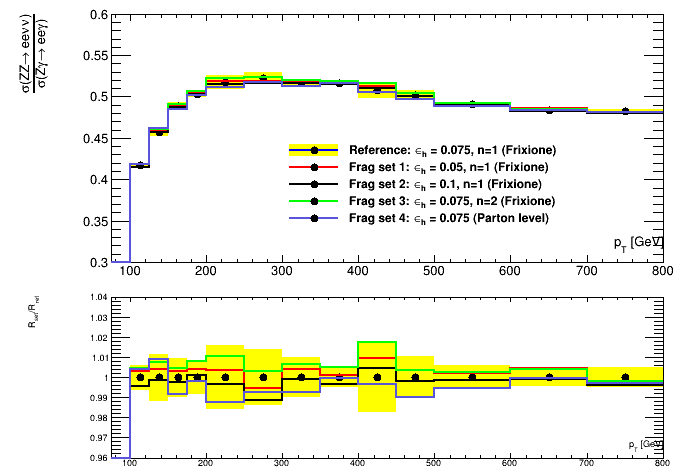
\includegraphics[width=0.7\textwidth]{frag.png}
	\caption{$R$ distribution as a function of $p_T$, showing the uncertainty due to variation of photon isolation parameters $\epsilon_h$ and $n$ in the smooth cone isolation procedure (Frixione), and $\epsilon_h$ in the photon isolation procedure. The lower panel shows the relative deviation of the varied sets from the central value, as well as the uncertainty band.}
	\label{fig:photon_frag}
\end{figure}

The uncertainty is calculated from the four sets listed in Figure \ref{fig:photon_frag}:
\begin{equation}
\begin{split}
\delta R_i &= |R_i - R_{ref}| \hspace{2cm}  i \in (1,2,3,4)\\
\delta R &= \sqrt{\max_{i=1,2,3}(\delta R_i)^2 + (\delta R_4)^2}
\end{split}
\end{equation}
as the effects assessed by changing the isolation definition in set 4, and varying the parameters in sets 1-3 are different.\\
The uncertainty is $< 2\%$ over the whole $p_T$ range.

\chapter{Additional Figures}
\begin{figure}[H]
\centering
	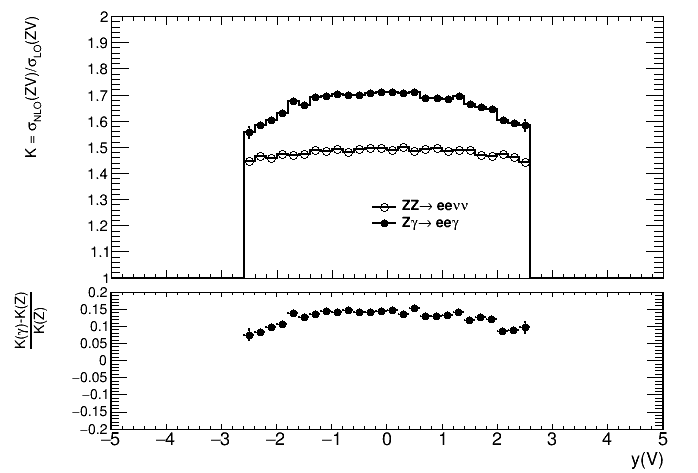
\includegraphics[width=0.7\textwidth]{K_y.png}
	\caption{K factor as a function of rapidity}
	\label{fig:K_y}
\end{figure}
\begin{figure}[H]
\centering
	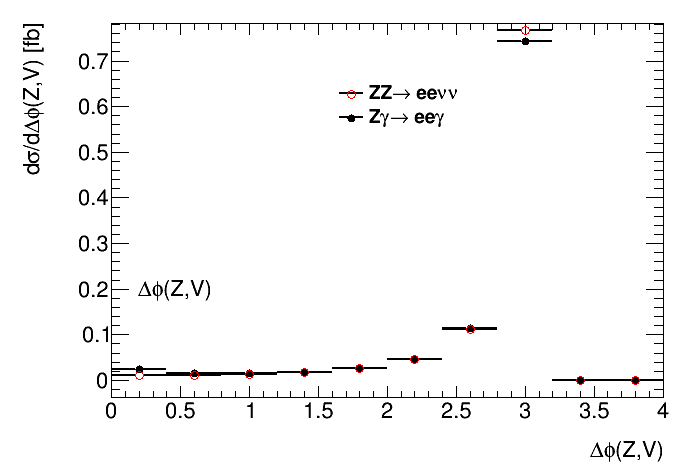
\includegraphics[width=0.7\textwidth]{dphi.png}
	\caption{dphi(Z,V)}
	\label{fig:dphi}
\end{figure}
\begin{figure}[H]
\centering
	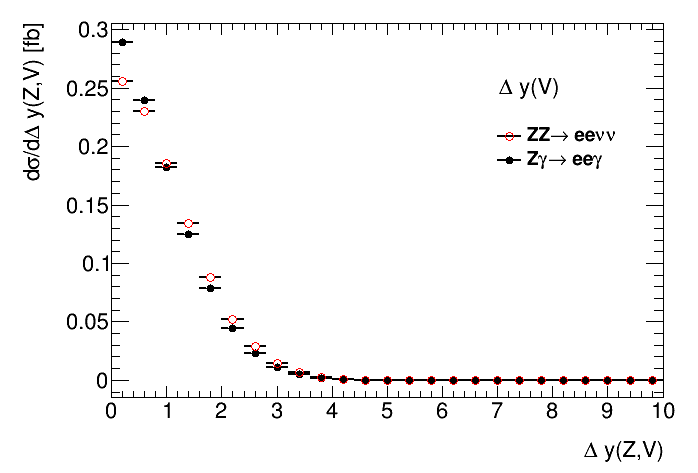
\includegraphics[width=0.7\textwidth]{dy.png}
	\caption{dy(Z,V)}
\end{figure}


%Bibliography
\begin{thebibliography}{9}
%1
\bibitem{SM}
	PBS NOVA, Fermilab, Office of Science, United States Department of Energy, Particle Data Group.

%2	
\bibitem{confinement}
\textbf{J. Greensite (2011)}. An introduction to the confinement problem. Springer. ISBN 978-3-642-14381-6.

%3
\bibitem{Higgs}
	\textbf{ATLAS Collaboration}, Observation of a New Particle in the Search for the Standard Model Higgs boson with the ATLAS detector at the LHC, \href{https://arxiv.org/pdf/1207.7214.pdf}{\texttt{arXiv:1207.7214}}

%4
\bibitem{galaxy}
	\textbf{Begeman, K. G., Broeils, A. H., Sanders, R. H.}, Extended rotation curves of spiral galaxies - Dark haloes and modified dynamics, Monthly Notices of the Royal Astronomical Society (ISSN 0035-8711), vol. 249, April 1, 1991, p. 523-537.
	
%5
\bibitem{DM_searches}
\textbf{Felix Kalhoefer}, Review of LHC Dark Matter searches, \href{https://arxiv.org/pdf/1702.02430.pdf}{\texttt{arXiv:1702.0243}}

\bibitem{mono_j}
\textbf{Philip Harris, Valentin V. Khoze, Michael Spannowsky, Ciaran Williams}, Closing up on Dark Sectors at Colliders: from 14 to 100 TeV, \href{https://arxiv.org/abs/1509.02904}{\texttt{arXiv:1509.02904}}

\bibitem{mono_V}
\textbf{Jing-Yuan, Edward W. Kolb, Lian-Tao Wang}, Dark matter coupling to electroweak gauge and Higgs bosons: an effective field theory approach, \href{https://arxiv.org/pdf/1305.0021}{\texttt{arXiv:1305.0021}}

\bibitem{mono_h}
\textbf{ATLAS Collaboration}, Search for dark matter produced in association with a Higgs boson decaying to two bottom quarks in pp collisions at $\sqrt{s} = 8$ TeV with the ATLAS detector, \href{https://arxiv.org/pdf/1510.06218}{\texttt{arXiv:1510.06218}}

\bibitem{MCFM}
\textbf{John Campbell, Keith Ellis, Walter Giele, Ciaran Williams},	Monte Carlo for FeMtobarn processes (MCFM) v8.0 User Manual, \url{https://mcfm.fnal.gov/}


\bibitem{ZH_ATLAS}
	\textbf{ATLAS Collaboration}, Search for an invisibly decaying Higgs boson or dark matter candidates produced in association with a Z boson in pp collisions at $\sqrt{s}$ = 13 TeV with the ATLAS detector, \texttt{arXiv:1708.09624}
	

\bibitem{gammajet}
	\textit{Using $\gamma +$ jets to calibrate the Standard Model $Z(\rightarrow \nu\nu)+$ jets background to new processes at the LHC}\\
	\textbf{S. Ask, M. A. Parker, T. Sandoval, M. E. Shea, W. J. Stirling}\\
Cavendish Laboratory, University of Cambridge, CB3 0HE, UK; 2011\\
	\texttt{[arXiv:1107.2803]}

\bibitem{Z_coupling}
	\textit{2017 Review of Particle Physics - Particle Listings}\\
	\textbf{C. Patrignani \textit{et al}. (Particle Data Group)}\\
	Chin. Phys. C, 40, 100001 (2016)
	
\bibitem{precise_scale}
	\textit{Precise predictions for $V$+jets dark matter backgrounds}\\
	\textbf{J.M. Lindert, S. Pozzorini, et al.}\\
	\texttt{arXiv:1705.04664}
	
\bibitem{CT14}
	\textit{New parton distribution functions from a global analysis of quantum chromodynamics}\\
	\textbf{Sayipjamal Dulat, Tie Jiun Hou, Jun Gao, Marco Guzzi, Joey Huston, P. Nadolsky, Jon Pumplin, Carl Schmidt, Daniel Stump, C. P. Yuan}\\
	\texttt{arXiv:1506.07443}

\bibitem{PDF4}
	\textit{PDF4LHC recommendations for LHC Run II}\\
	\texttt{[arXiv:1510.03865]}	
	
\bibitem{MMHT14}
	\textit{Parton distributions in the LHC era: MMHT 2014 PDFs}\\
	\textbf{L. A. Harland-Lang, A. D. Martin, P. Motylinski, R. S. Thorne}\\
	\texttt{arXiv:1412.3989}
	
\bibitem{NNPDF3}
	\textit{Parton distributions for the LHC Run II}\\
	\textbf{The NNPDF Collaboration: Richard D. Ball, Valerio Bertone, Stefano Carrazza, Christopher S. Deans, Luigi Del Debbio, Stefano Forte, Alberto Guffanti, Nathan P. Hartland, Jose I. Latorre, Juan Rojo, Maria Ubiali}\\
	\texttt{arXiv:1410.8849}
	
\bibitem{LHAPDF}
	\textit{LHAPDF6: parton density access in the LHC precision era}\\
	\textbf{Andy Buckley, James Ferrando, Stephen Lloyd, Karl Nordstrom, Ben Page, Martin Ruefenacht, Marek Schoenherr, Graeme Watt}\\
	\texttt{arXiv:1412.7420}

\bibitem{frixione}
	\textit{Isolated photons in perturbative QCD}\\	
	\textbf{S. Frixione}\\
	Phys. Lett.B429(1998)369–374, hep-ph/9801442
%	
%\bibitem{powheg}
%	POWHEG BOX - ZZ,WZ and WW production
%	\begin{itemize}
%	\item \textbf{P. Nason}\\
%	JHEP 0411 (2004) 040, hep-ph/0409146
%	\item \textbf{S. Frixione, P. Nason and C. Oleari}\\
%	JHEP 0711 (2007) 070, \texttt{arXiv:0709.2092}
%	\item \textbf{S. Alioli, P. Nason, C. Oleari and E. Re}\\
%	JHEP 1006 (2010) 043, \texttt{arXiv:1002.2581}
%	\item \textit{ZZ, WZ and W+W- production, including Gamma/Z interference, singly resonant contributions and interference for identical leptons}\\
%	\textbf{T. Melia, P. Nason, R. Rontsch, G. Zanderighi}\\
%	JHEP 1111 (2011) 078, \texttt{arXiv:1107.5051}
%	\item \textit{W+W-, WZ and ZZ production in the POWHEG-BOX-V2}\\
%	\textbf{P. Nason and G. Zanderighi}\\
%	Eur.Phys.J. C74 (2014) 2702, \texttt{arXiv:1311.1365}
%	\end{itemize}
%	
%\bibitem{pythia}
%	\textit{PYTHIA 8.1}\\
%	\textbf{T. Sjöstrand, S. Mrenna and P. Skands}\\
%	JHEP05 (2006) 026, Comput. Phys. Comm. 178 (2008) 852. 
%	
%\bibitem{CT10}
%	\textit{New parton distributions for collider physics}
%	\textbf{Hung-Liang Lai, Marco Guzzi, Joey Huston, Zhao Li, Pavel M. Nadolsky, Jon Pumplin, C.-P. Yuan}
%	\texttt{arXiv:1007.2241}
%	
%\bibitem{MSTW2008}
%	\textit{Parton distributions for the LHC}\\
%	\textbf{A.D. Martin, W.J. Stirling, R.S. Thorne, G. Watt}
%	\texttt{arXiv:0901.0002}
	
\end{thebibliography}
\end{document}

%\subsection{Effect of Lepton Cuts}
%To check the effects of lepton cuts on the ratio, samples with the same parameters as those in Table \ref{table:default} are generated. However, we relax the cuts on leptons. Both the leading and subleading lepton should have $p_T > 5$ GeV, and $\eta <$ 10. In the lower $p_T$ regions, the cross section falls by nearly half in both processes. The ratio is affected by up to 15\% as seen in Figure \ref{fig:lepcut}, and therefore for all following studies the lepton cuts are applied as they emulate the experimental cuts needed in the analysis.
%\begin{figure}[H]
%\centering
%	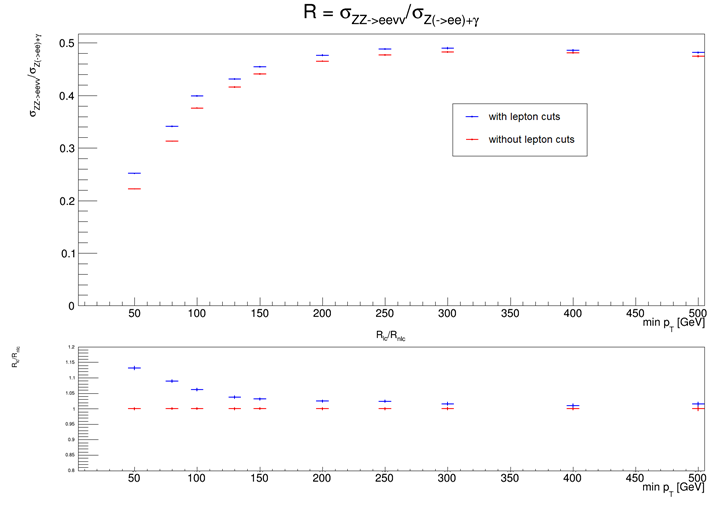
\includegraphics[width = 0.8\linewidth]{lep_cuts.png}
%	\caption{Comparison of reference the $R$ distribution to the $R$ distribution without lepton cuts}
%	\label{fig:lepcut}
%\end{figure}